\section{Results}

\subsection{APIC}

We evaluated the performance of the APIC method with different particle counts. Figure~\ref{fig:apic_comparison} shows simulation snapshots at three resolutions—1000, 4000, and 8000 particles—demonstrating how the method handles fluid detail, stability, and distribution over time. Each subfigure compares the final state of the fluid, and highlights how increasing the number of particles leads to smoother, more detailed results.

\begin{figure*}[h]
    \centering
    \begin{subfigure}[b]{0.2\textwidth}
        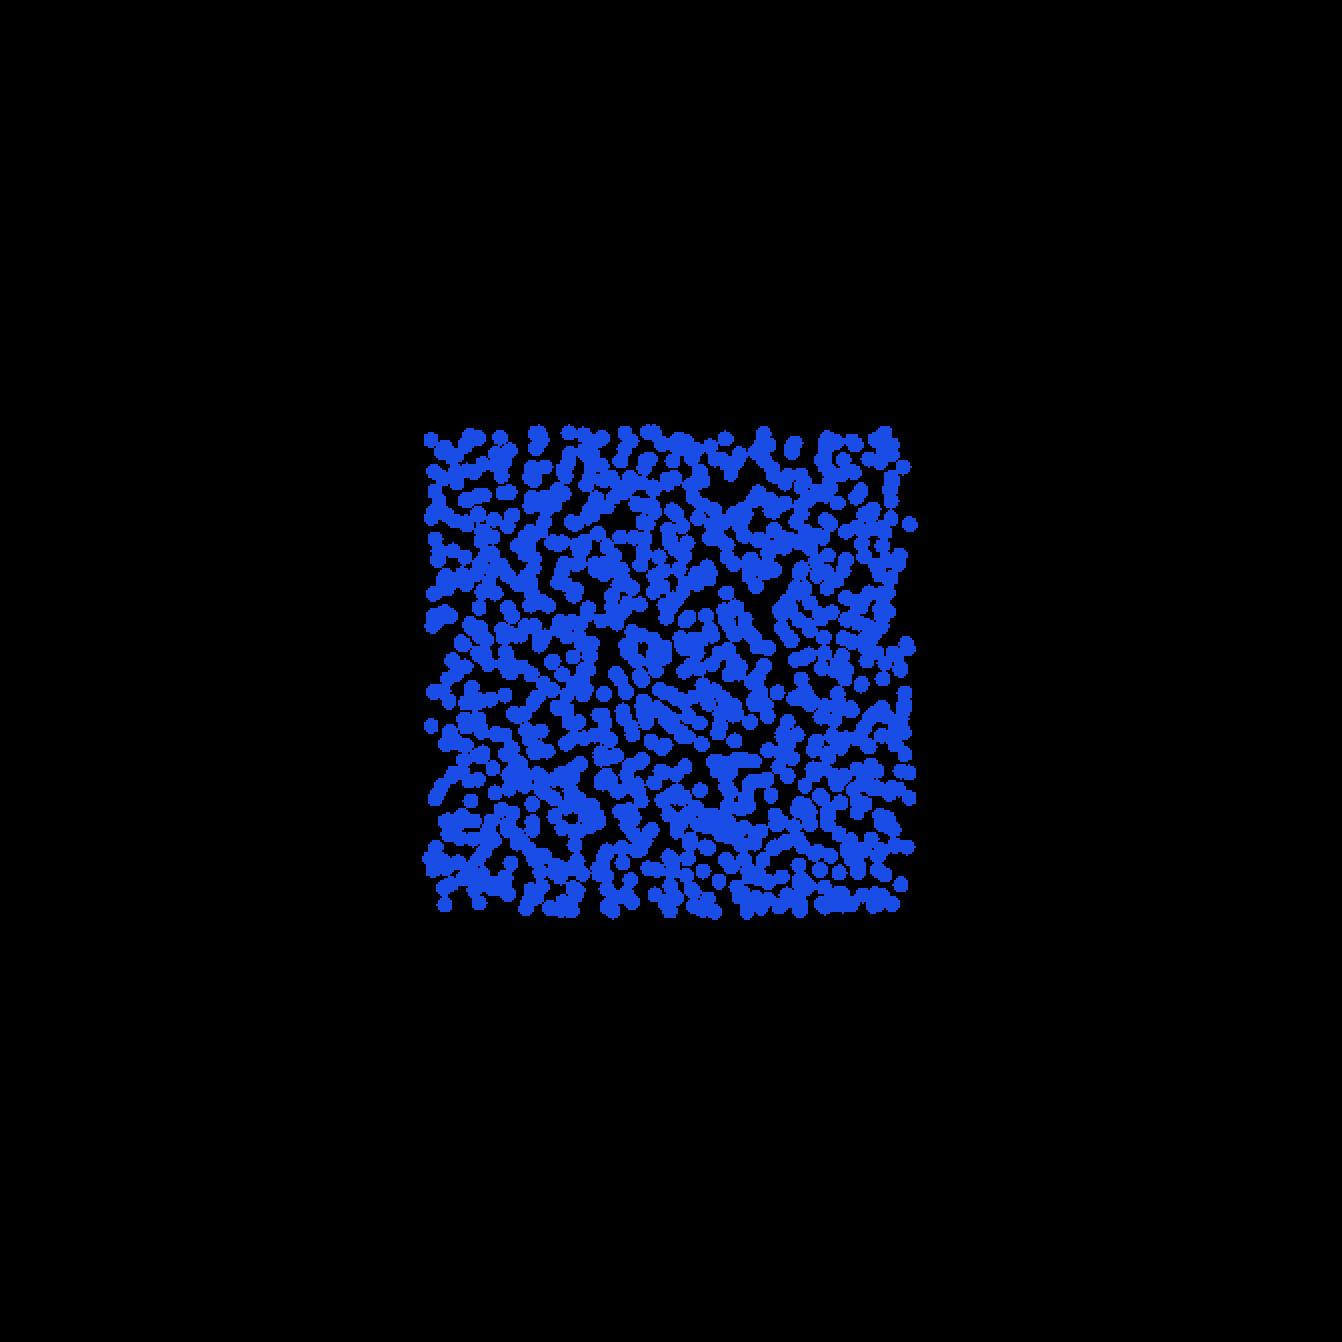
\includegraphics[width=\textwidth]{figures/apic1000_init.png}
        \caption{1000 initial particles}
    \end{subfigure}
    \begin{subfigure}[b]{0.2\textwidth}
        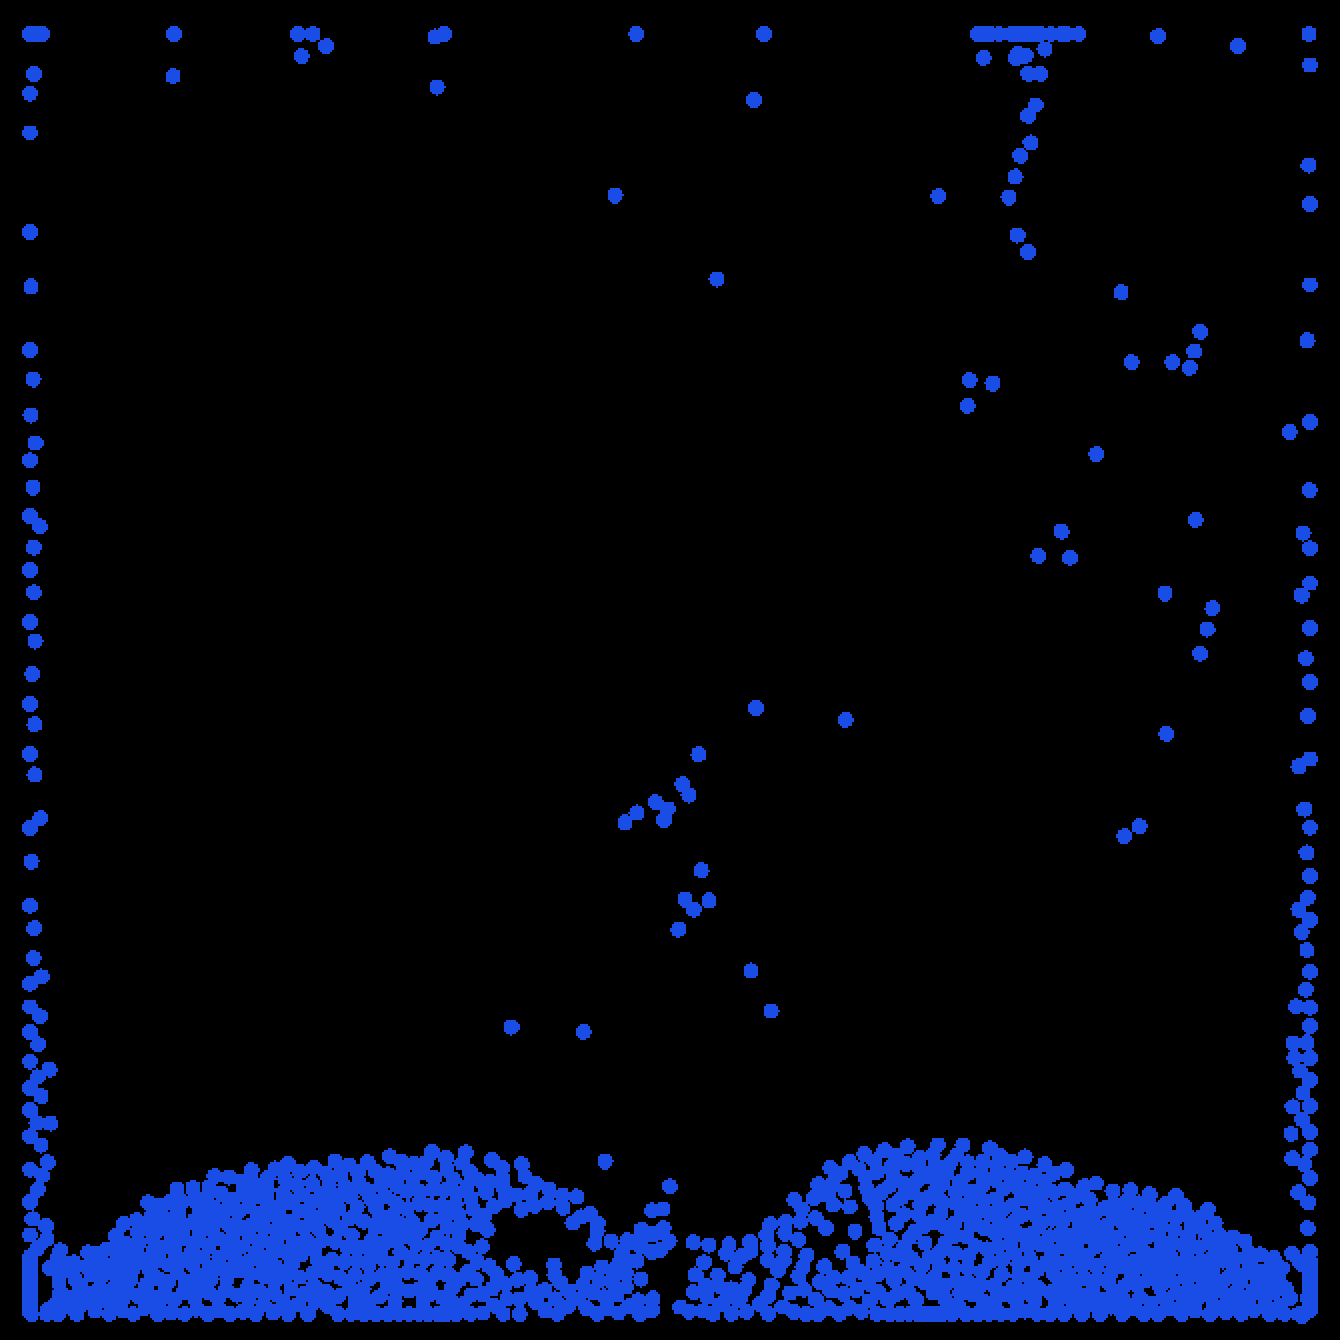
\includegraphics[width=\textwidth]{figures/apic1000.png}
        \caption{1000 particles}
    \end{subfigure}
    \begin{subfigure}[b]{0.2\textwidth}
        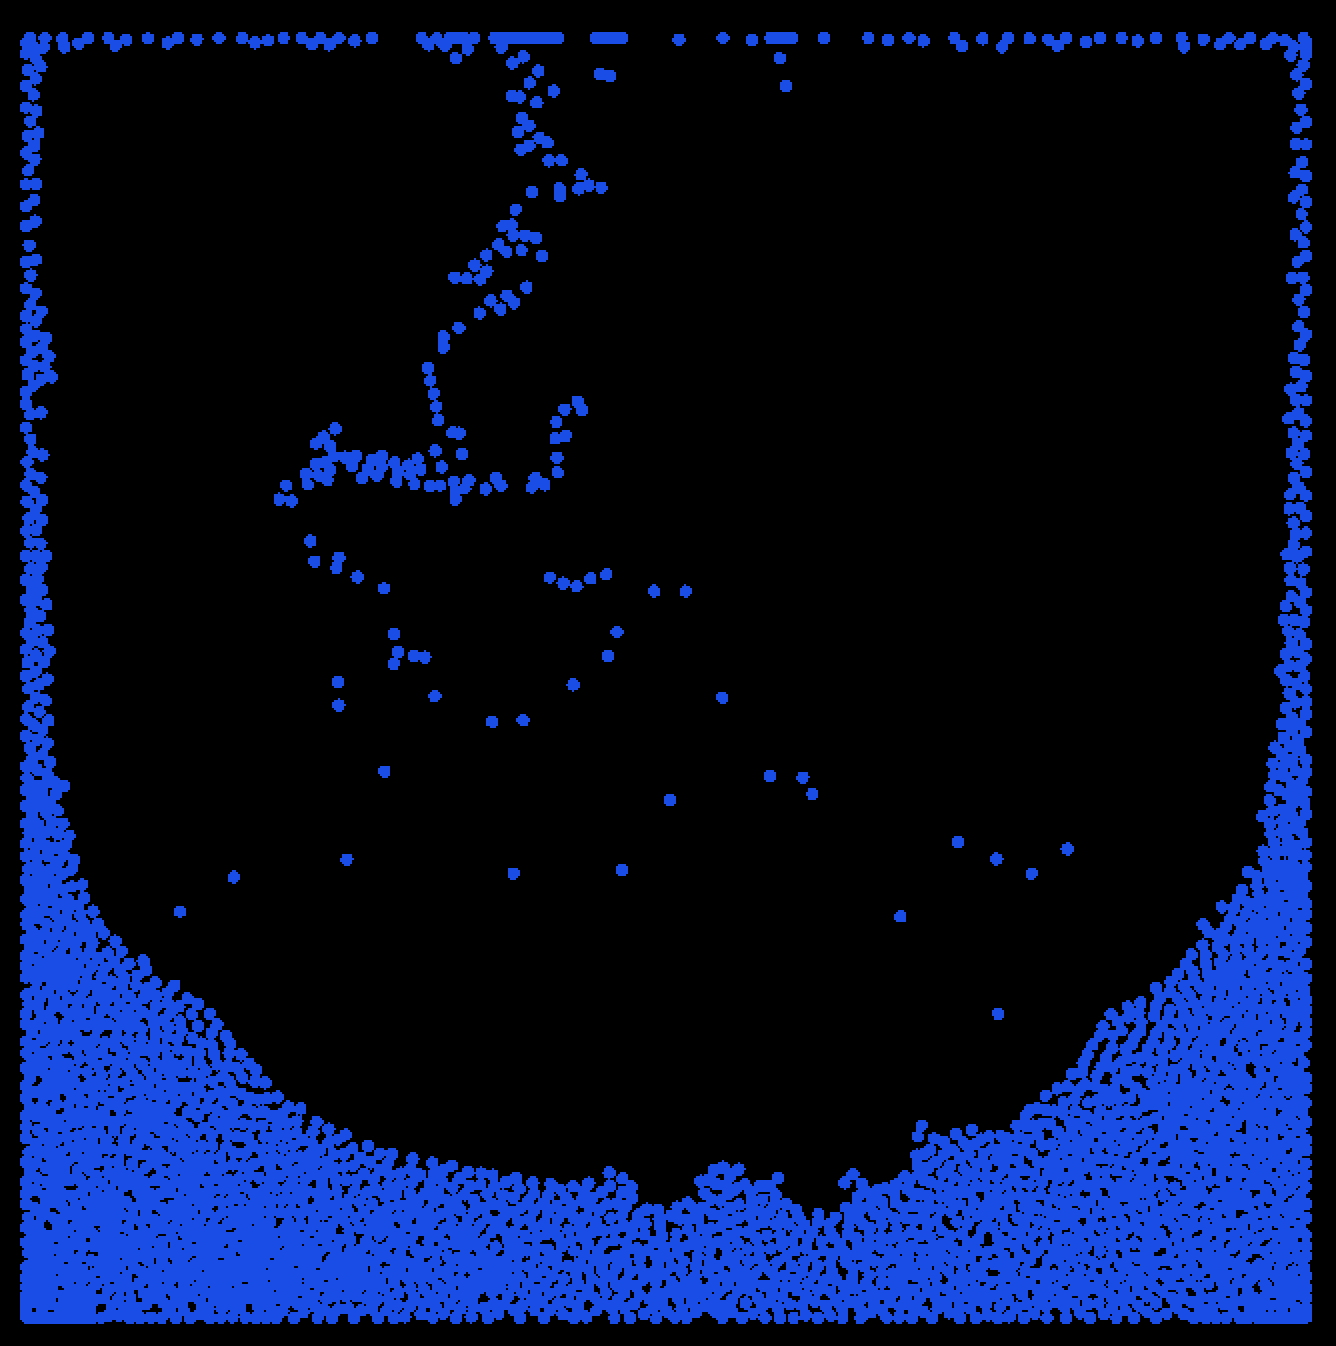
\includegraphics[width=\textwidth]{figures/apic4000.png}
        \caption{4000 particles}
    \end{subfigure}
    \begin{subfigure}[b]{0.2\textwidth}
        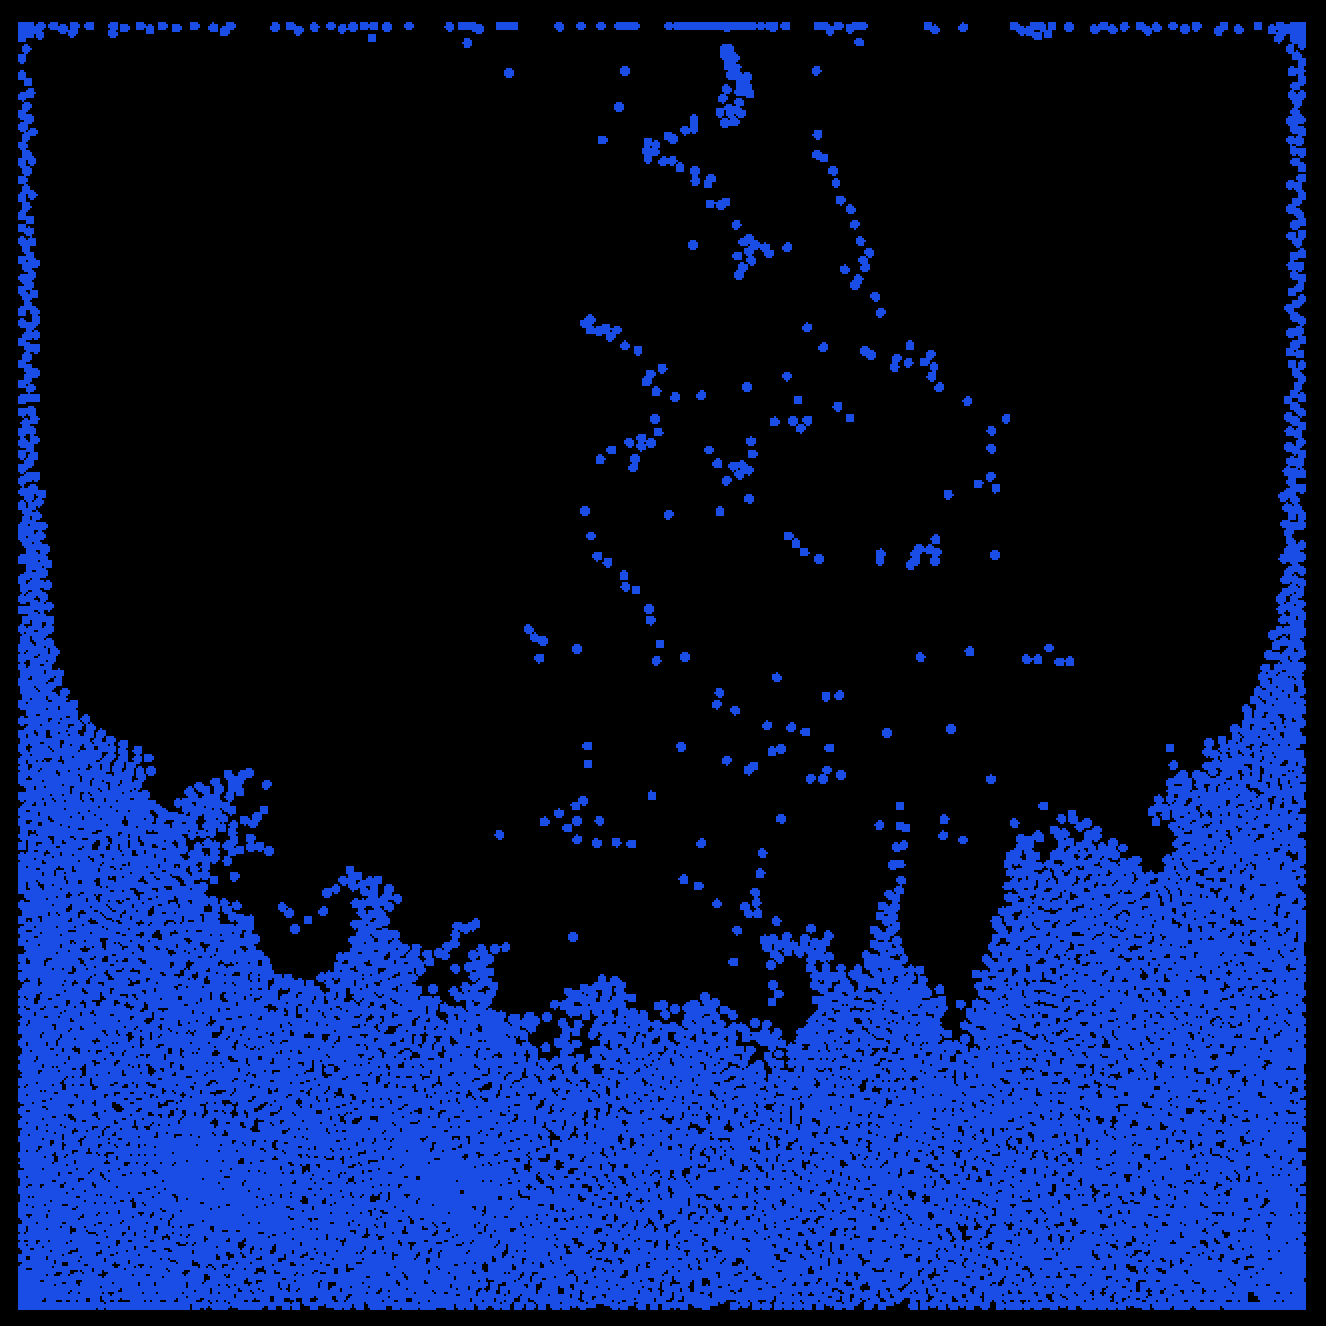
\includegraphics[width=\textwidth]{figures/apic8000.png}
        \caption{8000 particles}
    \end{subfigure}
    \caption{Comparison of APIC simulation results with increasing particle counts. 
    (a) shows the initial particle configuration, where all particles are placed in the center of the domain. 
    (b)–(d) show the simulation at the moment particles start to fall under gravity.}
    \label{fig:apic_comparison}
\end{figure*}